% \documentclass[handout]{beamer}
\documentclass{beamer}

\mode<presentation>
{
  \usetheme{ANLBlue}
  % \usefonttheme[onlymath]{serif}
  % \usetheme{Singapore}
  % \usetheme{Warsaw}
  % \usetheme{Malmoe}
  % \useinnertheme{circles}
  % \useoutertheme{infolines}
  % \useinnertheme{rounded}

  \setbeamercovered{transparent=20}
}

\usepackage[english]{babel}
\usepackage[latin1]{inputenc}
\usepackage{alltt,listings,multirow,ulem,siunitx}
\usepackage[absolute,overlay]{textpos}
\TPGrid{1}{1}
\usepackage{pdfpages}
\usepackage{ulem}
\usepackage{multimedia}
\usepackage{multicol}
\newcommand\hmmax{0}
\newcommand\bmmax{0}
\usepackage{bm}
\usepackage{comment}
\usepackage{subcaption}

% font definitions, try \usepackage{ae} instead of the following
% three lines if you don't like this look
\usepackage{mathptmx}
\usepackage[scaled=.90]{helvet}
% \usepackage{courier}
\usepackage[T1]{fontenc}
\usepackage{tikz}
\usetikzlibrary{decorations.pathreplacing}
\usetikzlibrary{shadows,arrows,shapes.misc,shapes.arrows,shapes.multipart,arrows,decorations.pathmorphing,backgrounds,positioning,fit,petri,calc,shadows,chains,matrix}

\newcommand\vvec{\bm v}
\newcommand\bvec{\bm b}
\newcommand\bxk{\bvec_0 \times \kappa_0 \cdot \nabla}
\newcommand\delp{\nabla_\perp}

% \usepackage{pgfpages}
% \pgfpagesuselayout{4 on 1}[a4paper,landscape,border shrink=5mm]

\usepackage{JedMacros}

\newcommand{\timeR}{t_{\mathrm{R}}}
\newcommand{\timeW}{t_{\mathrm{W}}}
\newcommand{\mglevel}{\ensuremath{\ell}}
\newcommand{\mglevelcp}{\ensuremath{\mglevel_{\mathrm{cp}}}}
\newcommand{\mglevelcoarse}{\ensuremath{\mglevel_{\mathrm{coarse}}}}
\newcommand{\mglevelfine}{\ensuremath{\mglevel_{\mathrm{fine}}}}

%solution and residual
\newcommand{\vx}{\ensuremath{x}}
\newcommand{\vc}{\ensuremath{\hat{x}}}
\newcommand{\vr}{\ensuremath{r}}
\newcommand{\vb}{\ensuremath{b}}

%operators
\newcommand{\vA}{\ensuremath{A}}
\newcommand{\vP}{\ensuremath{I_H^h}}
\newcommand{\vS}{\ensuremath{S}}
\newcommand{\vR}{\ensuremath{I_h^H}}
\newcommand{\vI}{\ensuremath{\hat I_h^H}}
\newcommand{\vV}{\ensuremath{\mathbf{V}}}
\newcommand{\vF}{\ensuremath{F}}
\newcommand{\vtau}{\ensuremath{\mathbf{\tau}}}


\title{PETSc software development pains and gains}
\author{Satish Balay, Jed Brown, Matt Knepley, Lois McInnes, Jason Sarich, Barry Smith}

% - Use the \inst command only if there are several affiliations.
% - Keep it simple, no one is interested in your street address.
% \institute
% {
%   Mathematics and Computer Science Division \\ Argonne National Laboratory
% }

\date{IDEAS workshop \\[1em]
{\small This talk: \url{http://59A2.org/files/20140930-PETSc.pdf}}}

% This is only inserted into the PDF information catalog. Can be left
% out.
\subject{Talks}


% If you have a file called "university-logo-filename.xxx", where xxx
% is a graphic format that can be processed by latex or pdflatex,
% resp., then you can add a logo as follows:

% \pgfdeclareimage[height=0.5cm]{university-logo}{university-logo-filename}
% \logo{\pgfuseimage{university-logo}}



% Delete this, if you do not want the table of contents to pop up at
% the beginning of each subsection:
% \AtBeginSubsection[]
% {
% \begin{frame}<beamer>
%   \frametitle{Outline}
%   \tableofcontents[currentsection,currentsubsection]
% \end{frame}
% }

% \AtBeginSection[]
% {
%   \begin{frame}<beamer>
%     \frametitle{Outline}
%     \tableofcontents[currentsection]
%   \end{frame}
% }

% If you wish to uncover everything in a step-wise fashion, uncomment
% the following command:

% \beamerdefaultoverlayspecification{<+->}

\begin{document}
\lstset{language=C}
\normalem

\begin{frame}
  \titlepage
\end{frame}

\begin{frame}{Interoperability Headaches}
  \begin{itemize}
  \item "libraries" that are not libraries
    \begin{itemize}
    \item too many assumptions
    \item tangled build process
    \item manual intervention necessary -- not designed for automation
    \item different process for different architectures
    \end{itemize}
  \item cyclic dependencies
    \begin{itemize}
    \item some hard to break without shared library plugins
    \end{itemize}
  \item broken environments, system software, compilers/wrappers
  \item lack of test suites sufficient to enable rapidly upgrading with confidence
  \item projects should use semantic versioning, but will break APIs periodically
  \item inextensible interfaces
  \item incompatible ABI under standard API (MPICH/Open MPI, LAPACK/ESSL)
  \end{itemize}
\end{frame}

\begin{frame}{Criteria for Success}
  \begin{itemize}
  \item predictable and reliable
    \begin{itemize}
    \item no interest in fancy features like LTO/Whole Program Optimization
    \item clear and accurate diagnostics
      \begin{itemize}
      \item can't trust any of them now, so I look at assembly regularly
      \end{itemize}
    \item no interest in pattern-match optimizations (triple-loop to GEMM)
    \end{itemize}
  \item Debuggable performance
    \begin{itemize}
    \item ability to audit memory locality and similar effects
    \item performance reproducibility (at least as an option) is useful
    \item application users rarely understand
      \begin{itemize}
      \item performance bottlenecks for their software
      \item fundamental limitations of the algorithms and hardware
      \item not just "clueless grad students"; includes many INCITE/ALCC awardees
      \end{itemize}
    \end{itemize}
  \item user customization without inline modification
  \end{itemize}
\end{frame}

\begin{frame}{Current practice for building}
  \begin{itemize}
  \item PETSc uses Python configuration and GNU Make build system
    \begin{itemize}
    \item 2 second incremental rebuilds
    \item many developers use ccache for switching branches
    \end{itemize}
  \item Python used for conditional compilation to preserve legacy system
    \begin{itemize}
    \item could easily switch to pure GNU Make for build
    \end{itemize}
  \item we maintain option of building with CMake
    \begin{itemize}
    \item used to be default build
    \item users reported many problems (some reported upstream as bugs)
    \item inexplicable hangs and "error code 256"
    \item poor diagnostics, exposes less parallelism than GNU Make
    \end{itemize}
  \end{itemize}
\end{frame}

\begin{frame}{Documentation and Testing}
  \begin{itemize}
  \item Documentation
    \begin{itemize}
    \item {\bf sowing} for man pages and generating Fortran bindings
      \begin{itemize}
      \item old and crufty, but gets the job done
      \item generating Fortran bindings is global and takes several
        seconds, problem for incremental rebuilds
      \end{itemize}
    \item \LaTeX{} for users manual, with scripts to insert links to website
    \item would like more web-friendly manual, man-page integration
      \begin{itemize}
      \item not happy with Doxygen; Fortran stubs would require custom code
      \end{itemize}
    \end{itemize}
  \item Testing
    \begin{itemize}
    \item daily or diurnal testing on \texttt{master} and \texttt{next}
    \item results summarized on web page
    \item too many false positives from floating point variability
      \begin{itemize}
      \item hard to avoid regression tests instead of unit tests
      % \item variable number of iterations needs fuzzy matching
      \end{itemize}
    \item need to build fewer executables to stay within quota
      \begin{itemize}
      \item \texttt{-Dmain=snes\_ex19} tricks for C; more intrusive for Fortran
      \end{itemize}
    \item Should run tests in parallel, but need to stay within resource limits
    \item GPUs not virtualized; multi-GPU tests need special machines
    \item MPICH won't fix 1000x performance regression for over-subscription, \texttt{ch3:sock} deprecated
      % so any test with more MPI ranks than cores needs a special build of
      % MPICH (using deprecated ch3:sock) so that an individual test can
      % complete in ~1 second instead of many minutes.
    \end{itemize}
  \end{itemize}
\end{frame}

\begin{frame}{External packages}
  \begin{itemize}
  \item can build external packages via \texttt{-{}-download-package}
  \item also support \text{-{}-with-package-dir=/path/to/my/install}
  \item some packages are abandoned/unmaintained upstream, but need critical bug fixes
    \begin{itemize}
    \item we maintain patches, though we don't want to
    \item some people use their own copies, encounter the bugs, and report them to us
    \end{itemize}
  \item shared vs static libs for external packages
    \begin{itemize}
    \item symbol conflicts due to lack of namespacing
    \item not following shared library rules
    \end{itemize}
  \item pkg-config not sufficient for multiple prefixes/configurations
  \item every package specifies configure-time options differently
    \begin{itemize}
    \item which MPI, 64-bit integers, real/complex, single/double/quad
    \item no way to check for compatibility
    \end{itemize}
  \end{itemize}
\end{frame}

\begin{frame}{Other topics}
  \begin{itemize}
  \item don't compromise on usability
  \item plugins are a fantastic model
    \begin{itemize}
    \item some facilities all but prevent them by insisting on static linking
    \end{itemize}
  \item too many broken tools
    \begin{itemize}
    \item compiler wrappers that don't return error codes
    \item compilers that crash on 1000-line plain C source
    \item MPI implementation that claims to implement MPI-3, but has critical bugs in MPI-2 implementation sitting in tickets for a decade
    \end{itemize}
  \item computing centers that buy the latest hardware, but install a 10-year old software stack ignorant of a 17-year old standard
  \item still can't assume C99
    \begin{itemize}
    \item we maintain hybrid C and C++ code, but some features conflict
    \end{itemize}
  \end{itemize}
\end{frame}

\begin{frame}{Git repository workflow}
  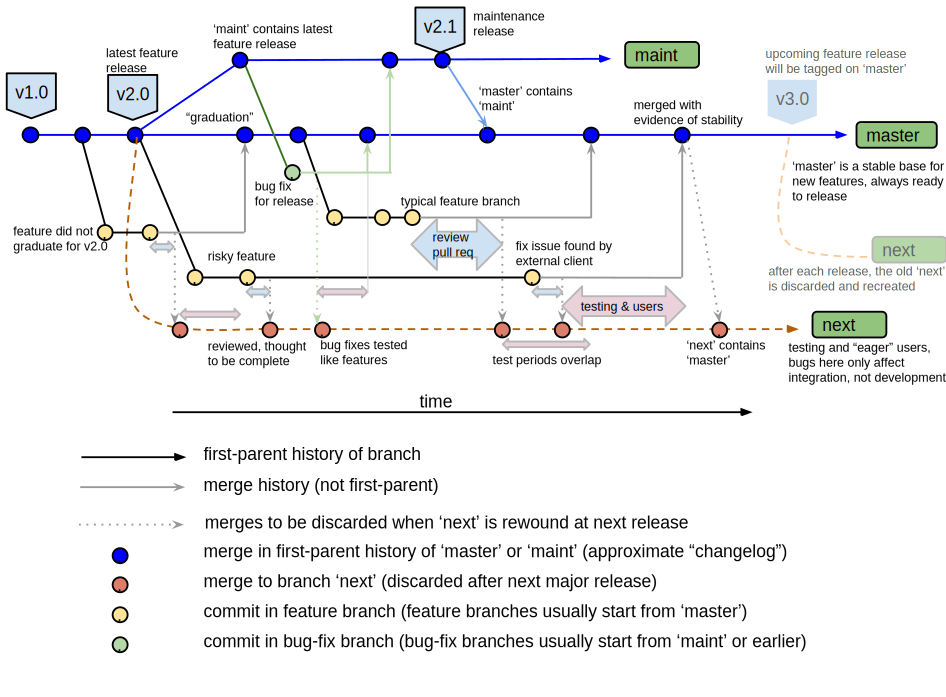
\includegraphics[width=\textwidth]{figures/simplified-gitworkflows7.png}
\end{frame}


\end{document}
